% PDF p. 83
\subsection{指数映射}
\subsubsection{双曲面（洛伦兹）模型中的指数映射}
指数映射是研究可微流形的重要工具。在经典微积分中，指数函数可定义为泰勒级数
\[
  \exp(x)=\sum_{k=0}^{\infty}\frac{x^k}{k!},
\]
% PDF p. 84
\begin{figure}[htbp]
  \centering
  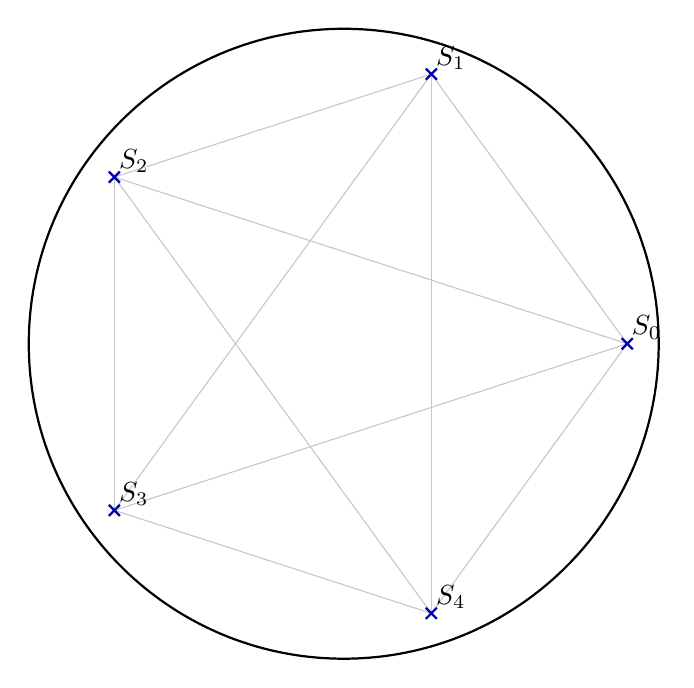
\begin{tikzpicture}[x=4cm,y=4cm]
  \draw[thick] (0,0) circle (1);
  \foreach \k in {0,...,4} {
    \coordinate (p\k) at ({72*\k}:.9);
  }
  \foreach \i in {0,...,4} {
    \foreach \j in {0,...,4} {
      \ifnum\i<\j
        \draw[black!22] (p\i)--(p\j);
      \fi
    }
  }
  \foreach \k in {0,...,4} {
    \draw[blue!70!black,thick]
      ([shift={(-2pt,-2pt)}]p\k)--([shift={(2pt,2pt)}]p\k)
      ([shift={(-2pt,2pt)}]p\k)--([shift={(2pt,-2pt)}]p\k);
    \node[above right,inner sep=1.5pt] at (p\k) {$S_{\k}$};
  }
\end{tikzpicture}

  \FigureCaption{2.5}{庞加莱圆盘中的五分类单元星形树。}
\end{figure}
也可以定义为下列微分方程的解。
\begin{equation*}
  \dot y=y.
  \tag{2.110}\label{eq:2.110}
\end{equation*}
经典指数函数定义在实直线或复平面上。为了将其推广到其他流形，按照式~\eqref{eq:2.110} 的启发，函数的自变量应为切向量。因此，首先定义双曲空间的切空间。

\begin{statement}{定义 2.8}{双曲空间的切空间}
在每个点 $x\in\mathbb H^n$，切空间定义为
\begin{equation*}
  T_x\mathbb H^n=\{v\in\R^{n+1}:\langle v,x\rangle=0\}.
  \tag{2.111}\label{eq:2.111}
\end{equation*}
图~\ref{fig:2.6} 展示了庞加莱圆盘（黑色圆）中的切空间 $T_x\mathbb H^2$。圆盘内的点 $x$ 表示双曲平面 $\mathbb H^2$ 中的位置。
\begin{itemize}
  \item 灰色虚线为经过 $x$ 的半径。
  \item 两个箭头 $v_1,v_2$ 张成\textbf{切空间} $T_x\mathbb H^2$。在流形上从 $x$ 出发的任意无穷小运动方向，都是这两个箭头的线性组合。
\end{itemize}
由于庞加莱模型是共形的，切空间在该点可以按欧氏方式画出。标记 $T_x\mathbb H^2$ 表示这个二维平面。

% PDF p. 85
\begin{figure}[htbp]
  \centering
  \begin{tikzpicture}[x=3.1cm,y=3.1cm,>=Stealth]
  \draw[thick] (0,0) circle (1);
  \coordinate (x) at (.46,.46);
  \draw[dashed,black!52] (0,0)--(x);
  \draw[red!85!black,very thick,->] (x)--(.246,.674)
    node[above right,inner sep=2pt] {$v_1$};
  \draw[red!85!black,very thick,->] (x)--(.246,.246)
    node[above right,inner sep=2pt] {$v_2$};
  \fill (x) circle (1.3pt) node[above right,inner sep=2pt] {$x$};
  \node[red!85!black] at (.73,.24) {$T_x\mathbb H^2$};
\end{tikzpicture}

  \FigureCaption{2.6}{庞加莱圆盘中的切空间 $T_x\mathbb H^2$。}
\end{figure}
切向量 $v$ 的双曲范数定义如下。\translatornote{原书此处写作空间分量的欧氏范数。一般的双曲面切空间上，以下测地线公式用的是限制在切空间上的洛伦兹内积所诱导的范数。两种范数在 $x=(1,0,\ldots,0)$ 处相同。}
\[
  \lVert v\rVert=\sqrt{\langle v,v\rangle_{\mathrm{Euc}}}
  \qquad\text{（“空间分量”的通常欧氏范数）}.
\]

需要指出，洛伦兹内积 $\langle v,v\rangle$ 一般可能为正、为负或为零，但对 $x$ 处满足 $\langle x,v\rangle=0$ 的切向量 $v$，有 $\langle v,v\rangle\geq0$。因此 $\lVert v\rVert$ 为非负实数。

接下来刻画双曲面上的测地线。设初始点 $x\in\mathbb H^n$，初始切速度 $v\in T_x\mathbb H^n$。定义线性子空间 $V=\Span\{x,v\}\subseteq\R^{n+1}$。曲线 $\gamma(t)$ 由交集 $V\cap\mathbb H^n$ 给出。要求其参数化 $\gamma(t)\in V\cap\mathbb H^n$ 满足 $\gamma(0)=x$ 和 $\gamma'(0)=v$（图~\ref{fig:2.7}）。

换句话说，$\gamma(t)$ 必须满足下列条件。\translatornote{第一条不等式沿用原书。按双曲面的定义，曲线在面上应满足 $\langle\gamma(t),\gamma(t)\rangle=-1$，下文验证的也是等式。}
\[
  \langle\gamma(t),\gamma(t)\rangle\geq-1,\qquad
  \gamma(0)=x,\qquad
  \gamma'(0)=v.
\]
通过试算可以得到
\begin{equation*}
  \gamma(t)=\cosh(\alpha t)x+\sinh(\alpha t)\frac{v}{\lVert v\rVert}.
  \tag{2.112}\label{eq:2.112}
\end{equation*}
下面验证式~\eqref{eq:2.112} 定义的 $\gamma(t)$ 确实满足上述三个条件。

% PDF p. 86
\begin{figure}[htbp]
  \centering
  \begin{tikzpicture}
\begin{axis}[
  width=.72\linewidth,height=.48\linewidth,
  axis lines=left,xmin=-11,xmax=11,ymin=-5,ymax=105,
  xtick={-10,-7.5,-5,-2.5,0,2.5,5,7.5,10},
  ytick={0,20,40,60,80,100},
  tick label style={font=\scriptsize},label style={font=\small},
  xlabel={$x$ 轴},ylabel={$y$ 轴},
  grid=major,major grid style={black!12,dotted},
  legend pos=south west,legend style={font=\small},
  clip=false
]
  \draw[dashed,black!55] (axis cs:0,-5)--(axis cs:0,105);
  \draw[dashed,black!55] (axis cs:-11,0)--(axis cs:11,0);
  \addplot[blue!65!black,thick,domain=-10:10,samples=81]{x^2};
  \addlegendentry{$y=x^2$}
  \draw[green!60!black,line width=1.4pt]
    (axis cs:2.24,-7.3)--(axis cs:11.9,104);
  \fill[red!80!black] (axis cs:5.75,33.06) circle (1.5pt)
      node[right,inner sep=2pt] {$x$};
  \node[green!60!black,anchor=west] at (axis cs:9.22,69.5) {$v$};
  \node[anchor=west,font=\small] at (axis cs:7.85,42)
    {$\gamma(0)=x,\ \gamma'(0)=v$};
  \draw[orange!95!black,very thick,-{Stealth}]
    (axis cs:10.6,85.5)--(axis cs:9.46,89.5);
  \node[anchor=west,align=left,font=\small\bfseries] at (axis cs:10.65,85)
    {把一点映回\\流形。};
\end{axis}
\end{tikzpicture}

  \FigureCaption{2.7}{指数映射。}
\end{figure}
回顾
\[
  \cosh(t)=\frac{e^t+e^{-t}}2,\qquad
  \sinh(x)=\frac{e^x-e^{-x}}2.
\]
在 $t=0$ 时，
\[
  \gamma(0)=\cosh(0)x+\sinh(0)\frac{v}{\lVert v\rVert}=x+0=x.
\]
对式~\eqref{eq:2.112} 求导并在 $t=0$ 处计算。\translatornote{原书的 $\gamma'(t)$ 第一项缺少因子 $x$。该项在 $t=0$ 时为零。}
\[
  \gamma'(t)=\alpha\sinh(\alpha t)
       +\alpha\cosh(\alpha t)\frac{v}{\lVert v\rVert},
\]
从而
\[
  \gamma'(0)=\alpha\frac{v}{\lVert v\rVert}.
\]
若 $\alpha=\lVert v\rVert$，则 $\gamma'(0)=v$。把 $\alpha=\lVert v\rVert$ 代入式~\eqref{eq:2.112} 得
\begin{equation*}
  \gamma(t)=\cosh(\lVert v\rVert t)x
            +\sinh(\lVert v\rVert t)\frac{v}{\lVert v\rVert}.
  \tag{2.113}\label{eq:2.113}
\end{equation*}
最后，验证 $\langle\gamma(t),\gamma(t)\rangle=-1$。事实上，由式~\eqref{eq:2.113} 得
% PDF p. 87
\[
  \begin{aligned}
    \langle\gamma(t),\gamma(t)\rangle
      &=\cosh^2(\lVert v\rVert t)\langle x,x\rangle\\
      &\quad+2\cosh(\lVert v\rVert t)\sinh(\lVert v\rVert t)
             \left\langle x,\frac{v}{\lVert v\rVert}\right\rangle\\
      &\quad+\sinh^2(\lVert v\rVert t)
             \left\langle\frac{v}{\lVert v\rVert},
                         \frac{v}{\lVert v\rVert}\right\rangle\\
      &=-\cosh^2(\lVert v\rVert t)+\sinh^2(\lVert v\rVert t)\\
      &=-\left(\frac{e^{\lVert v\rVert t}+e^{-\lVert v\rVert t}}2\right)^2
        +\left(\frac{e^{\lVert v\rVert t}-e^{-\lVert v\rVert t}}2\right)^2\\
      &=-\frac{e^{2\lVert v\rVert t}+2+e^{-2\lVert v\rVert t}}4
        +\frac{e^{2\lVert v\rVert t}-2+e^{-2\lVert v\rVert t}}4\\
      &=-\frac12-\frac12=-1.
  \end{aligned}
\]
这表明曲线 $\gamma(t)$ 始终位于 $\mathbb H^n$ 上。由于 $\gamma(t)$ 正是从 $x$ 以速度 $v$ 出发的唯一测地线，可以写成
\begin{equation*}
  \exp_x(tv)=\gamma(t).
  \tag{2.114}\label{eq:2.114}
\end{equation*}
取 $t=1$，得到从 $T_x\mathbb H^n$ 到 $\mathbb H^n$ 的\textbf{指数映射公式}
\begin{equation*}
  \exp_x(v)=\gamma(1)=\cosh(\lVert v\rVert)x+
            \sinh(\lVert v\rVert)\frac{v}{\lVert v\rVert}.
  \tag{2.115}\label{eq:2.115}
\end{equation*}
\textbf{特殊情形。}若 $v=0$，则 $\exp_x(0)=x$。

其中，$\cosh(\lVert v\rVert)$ 这一部分保证所得点仍在双曲面上，而 $\sinh(\lVert v\rVert)v/\lVert v\rVert$ 这一部分沿切向移动。
\end{statement}

\subsubsection{一般黎曼流形中的指数映射公式}
指数映射的\textbf{定义}对每个黎曼流形都相同。能实际写出的\textbf{闭式公式}取决于具体度量。双曲空间恰好有简单的闭式公式，庞加莱球和洛伦兹模型都有。对一般的黎曼流形，通常无法把 $\exp_x(v)$ 写成单个代数表达式，需要数值积分求解测地线方程。

\paragraph{普适定义}
对任一黎曼流形 $(M,g)$ 和任一基点 $x\in M$，
\[
  \exp_x(v)=\gamma_v(1),\qquad v\in T_xM,
\]
其中 $\gamma_v$ 是满足 $\gamma_v(0)=x$ 和 $\dot\gamma_v(0)=v$ 的\textbf{唯一测地线}。\translatornote{若流形不完备，指数映射只在那些使测地线能延拓到 $t=1$ 的初速度上有定义。}

因此，指数映射是指“从 $x$ 以初速度 $v$ 沿测地线出发，取其在时刻 1 的位置”。该定义\textbf{不要求}任何特殊度量。

\paragraph{随流形而变的是什么？}
要把定义化为\textbf{公式}，需要求解测地线常微分方程
\[
  \ddot\gamma^k(t)+\Gamma^k_{ij}(\gamma(t))\dot\gamma^i(t)\dot\gamma^j(t)=0.
\]

% PDF p. 88
\textbf{一般流形。}克里斯托费尔符号（Christoffel symbols）$\Gamma^k_{ij}$ 的形式随流形而异，因此在大多数情况下只能数值积分，得不到闭式。

\textbf{双曲空间有闭式（见第 2.9.7 节）。}对于常负曲率 $-1$，可得形式简洁的公式。
\begin{itemize}
  \item \textbf{庞加莱球 $\mathbb B^n$。}对于 $x=0$（球心），
    \[
      \exp_0(v)=\tanh(\lVert v\rVert)\frac{v}{\lVert v\rVert}.
    \]
    对于一般点 $x$，可写为莫比乌斯旋向量（Möbius gyrovector）公式
    \[
      \exp_x(v)=x\oplus\left(
       \tanh\left(\frac{\lambda_x\lVert v\rVert}{2}\right)
                \frac{v}{\lVert v\rVert}\right),\qquad
      \lambda_x=\frac{2}{1-\lVert x\rVert^2},
    \]
    其中 $\oplus$ 是莫比乌斯加法。
  \item \textbf{洛伦兹（双曲面）模型。}
    \[
      \exp_x(v)=\gamma(1)=\cosh(\lVert v\rVert)x+
             \sinh(\lVert v\rVert)\frac{v}{\lVert v\rVert}.
    \]
\end{itemize}
所以，定义处处相同，所能写出的代数表达式一般随流形而变。双曲空间恰好是具有简洁闭式的少数情形之一。

\subsection{对数映射（逆指数映射）}
\begin{statement}{定义 2.9}{对数映射（逆指数映射）}
对数映射（logarithmic map）定义为指数映射的逆。给定两点 $x,y\in\mathbb H^n$，将 $\log_x y$ 定义为满足 $y=\exp_x(v)$ 的唯一切向量 $v\in T_x\mathbb H^n$。在双曲面（洛伦兹）模型中，对数映射的计算公式为
\begin{equation*}
  \log_x y=d(x,y)\frac{y+\langle x,y\rangle x}
                       {\lVert y+\langle x,y\rangle x\rVert},
  \tag{2.116}\label{eq:2.116}
\end{equation*}
其中两点 $x,y\in\mathbb H^n$ 之间的双曲距离为
\begin{equation*}
  d(x,y)=\operatorname{arcosh}(-\langle x,y\rangle).
  \tag{2.117}\label{eq:2.117}
\end{equation*}

\textbf{证明。}回顾，沿切向量 $v\in T_x\mathbb H^n$ 的方向经过 $x\in\mathbb H^n$ 的测地线为
% PDF p. 89
\begin{equation*}
  \gamma(t)=\cosh(t)x+\sinh(t)\frac{v}{\lVert v\rVert},
  \tag{2.118}\label{eq:2.118}
\end{equation*}
其中 $t\in\R$ 为测地线参数，$\lVert v\rVert=\sqrt{\langle v,v\rangle}$ 为 $v$ 的范数。

由测地线的定义，在 $t=d(x,y)$ 时，$\gamma(t)$ 到达 $y$。于是由式~\eqref{eq:2.118} 得
\begin{equation*}
  y=\cosh\bigl(d(x,y)\bigr)x+\sinh\bigl(d(x,y)\bigr)\frac{v}{\lVert v\rVert}.
  \tag{2.119}\label{eq:2.119}
\end{equation*}
为从式~\eqref{eq:2.119} 求出 $v$，将右边的第一项移到左边。
\begin{equation*}
  y-\cosh\bigl(d(x,y)\bigr)x=\sinh\bigl(d(x,y)\bigr)\frac{v}{\lVert v\rVert}.
  \tag{2.120}\label{eq:2.120}
\end{equation*}
两边乘以 $\lVert v\rVert$，得到
\begin{equation*}
  \lVert v\rVert\bigl(y-\cosh(d(x,y))x\bigr)=\sinh\bigl(d(x,y)\bigr)v.
  \tag{2.121}\label{eq:2.121}
\end{equation*}
对式~\eqref{eq:2.121} 两边取范数，得到下式。\translatornote{式~\eqref{eq:2.122} 的右边按原书保留。由取范数的步骤可知，右边应加范数符号。}
\begin{equation*}
  \sinh\bigl(d(x,y)\bigr)=y-\cosh\bigl(d(x,y)\bigr)x,
  \tag{2.122}\label{eq:2.122}
\end{equation*}
从而
\begin{equation*}
  \frac{v}{\lVert v\rVert}
    =\frac{y-\cosh(d(x,y))x}{\lVert y-\cosh(d(x,y))x\rVert}.
  \tag{2.123}\label{eq:2.123}
\end{equation*}
直观上，$\lVert v\rVert=d(x,y)$，所以
\begin{equation*}
  v=d(x,y)\frac{y-\cosh(d(x,y))x}{\lVert y-\cosh(d(x,y))x\rVert}.
  \tag{2.124}\label{eq:2.124}
\end{equation*}
由式~\eqref{eq:2.117} 得
\begin{equation*}
  \cosh\bigl(d(x,y)\bigr)=-\langle x,y\rangle,
  \tag{2.125}\label{eq:2.125}
\end{equation*}
从而
\begin{equation*}
  y-\cosh\bigl(d(x,y)\bigr)x=y+\langle x,y\rangle x.
  \tag{2.126}\label{eq:2.126}
\end{equation*}
把式~\eqref{eq:2.126} 代入式~\eqref{eq:2.124} 得
% PDF p. 90
\begin{equation*}
  \log_x y=v=d(x,y)\frac{y+\langle x,y\rangle x}
                        {\lVert y+\langle x,y\rangle x\rVert}.
  \tag{2.127}\label{eq:2.127}
\end{equation*}
\end{statement}

\subsection{庞加莱球模型的指数映射和对数映射}
回顾，在曲率为 $-1$ 的庞加莱球模型中，$n$ 维双曲空间等同于开单位球
\[
  \mathbb B^n=\{x\in\R^n:\lVert x\rVert<1\},
\]
其中距离和测地线由黎曼度量
\[
  g_x=\lambda_x^2\delta,\qquad \lambda_x=\frac{2}{1-\lVert x\rVert^2}
\]
诱导，$\delta$ 是通常的欧氏度量。两个向量 $x,y\in\mathbb B^n$ 的“莫比乌斯加法”定义为
\begin{equation*}
  x\oplus y
    =\frac{(1+2\langle x,y\rangle+\lVert y\rVert^2)x+(1-\lVert x\rVert^2)y}
           {1+2\langle x,y\rangle+\lVert x\rVert^2\lVert y\rVert^2},
  \tag{2.128}\label{eq:2.128}
\end{equation*}
其中 $\langle\cdot,\cdot\rangle$ 是通常的欧氏点积。

\subsubsection{从原点出发的指数映射}
先研究从原点 $0$ 出发的映射。对 $v\in T_0\mathbb B^n\cong\R^n$，有
\begin{equation*}
  \exp_0(v)=\tanh(\lVert v\rVert)\frac{v}{\lVert v\rVert}.
  \tag{2.129}\label{eq:2.129}
\end{equation*}
若 $v=0$，则 $\exp_0(0)=0$。

\subsubsection{一般的指数映射}
对一般点 $x\in\mathbb B^n$ 及 $v\in T_x\mathbb B^n\cong\R^n$，可以用莫比乌斯加法表示指数映射。常见的一个公式为
\begin{equation*}
  \exp_x(v)=x\oplus\left(\tanh\left(\frac{\lambda_x}{2}\lVert v\rVert\right)\right)
               \frac{v}{\lVert v\rVert},
  \tag{2.130}\label{eq:2.130}
\end{equation*}
其中 $\lambda_x=2/(1-\lVert x\rVert^2)$。\translatornote{式~\eqref{eq:2.130} 依原书括号排印。按本节之前的莫比乌斯加法公式，$v/\lVert v\rVert$ 应乘在 $\tanh$ 项上，所得向量是 $\oplus$ 的第二个自变量。}

\Subheading{对数映射}
作为 $\exp_x$ 的逆映射，对应的对数映射 $\log_x y$ 对 $x,y\in\mathbb B^n$ 的表达式为
\begin{equation*}
  \log_x y=\frac{2}{\lambda_x}\tanh^{-1}\bigl(\lVert(-x)\oplus y\rVert\bigr)
             \frac{(-x)\oplus y}{\lVert(-x)\oplus y\rVert},
  \tag{2.131}\label{eq:2.131}
\end{equation*}
% PDF p. 91
其中 $(-x)\oplus y$ 是 $-x$ 与 $y$ 的莫比乌斯和，$\lVert(-x)\oplus y\rVert$ 是所得向量在 $\R^n$ 中的通常欧氏范数。
